\documentclass[english,10pt,aspectratio=169]{beamer}

\usepackage{amsmath} % load this before unicode-math
\usepackage{amssymb}
%\usepackage{unicode-math}

\usepackage{fontspec}
\setmonofont{JuliaMono}

\usefonttheme[onlymath]{serif}

\setlength{\parskip}{\smallskipamount}
\setlength{\parindent}{0pt}

%\setbeamersize{text margin left=5pt, text margin right=5pt}

\usepackage{amsmath}
\usepackage{amssymb}
\usepackage{braket}
\usepackage{mhchem}

\usepackage{minted}
\newminted{julia}{breaklines,fontsize=\scriptsize,texcomments=true}
\newminted{python}{breaklines,fontsize=\scriptsize,texcomments=true}
\newminted{bash}{breaklines,fontsize=\scriptsize,texcomments=true}
\newminted{text}{breaklines,fontsize=\scriptsize,texcomments=true}

\newcommand{\txtinline}[1]{\mintinline[fontsize=\scriptsize]{text}{#1}}
\newcommand{\jlinline}[1]{\mintinline[fontsize=\scriptsize]{julia}{#1}}

\definecolor{mintedbg}{rgb}{0.95,0.95,0.95}
\usepackage{mdframed}

%\BeforeBeginEnvironment{minted}{\begin{mdframed}[backgroundcolor=mintedbg]}
%\AfterEndEnvironment{minted}{\end{mdframed}}

\setcounter{secnumdepth}{3}
\setcounter{tocdepth}{3}

\makeatletter

 \newcommand\makebeamertitle{\frame{\maketitle}}%
 % (ERT) argument for the TOC
 \AtBeginDocument{%
   \let\origtableofcontents=\tableofcontents
   \def\tableofcontents{\@ifnextchar[{\origtableofcontents}{\gobbletableofcontents}}
   \def\gobbletableofcontents#1{\origtableofcontents}
 }

\makeatother

\usepackage{babel}

\begin{document}


\title{Recent CMD ITB Lab Research on\\
Density Functional Theory Software Development}
\author{Fadjar Fathurrahman}
\institute{
Engineering Physics \\
Institut Teknologi Bandung
}
\date{24 February 2022}

\frame{\titlepage}


\begin{frame}
\frametitle{Some background information}

My first exposure to first-principles calculations (around 2008-2010):
\begin{itemize}
\item ABINIT, CPMD, Quantum Espresso, PyQuante, ELK, ...
\item Asian CMD Workshop
\end{itemize}

Linux environment: configure, make, make install
Linking to libraries: BLAS, LAPACK

Learn DFT by using the softwares to do the calculations ...

I am still learning by now

\end{frame}



\begin{frame}
\frametitle{Course about DFT in TF ITB (2010)}

\begin{itemize}
\item Taught by Prof. Hermawan. Based on Prof. Arias course materials:
  \begin{itemize}
  \item Old website: {\footnotesize\url{https://dft.physics.cornell.edu/old-website/minicourse/}}
  \item New website: {\footnotesize\url{http://jdftx.org/PracticalDFT.html}}
  \end{itemize}
\item Using C programming language and Octave (a MATLAB clone)
\item Plane wave basis set and DFT++ formalism
\item radial atomic problem, H atom $\ce{H2}$ molecule in a box, Ge crystal (8 atoms in a
cubic unit cell, local pseudopotential), quantum dot (with harmonic potential confinement)
\end{itemize}

\end{frame}


\begin{frame}

Motivation:

\end{frame}


\begin{frame}
\frametitle{First try: plane wave pseudopotential code (2010-2012)}

During my master thesis, I decided to write my own density functional theory
based on plane wave and pseudopotential:

{\footnotesize\url{https://github.com/f-fathurrahman/ffr-pspw-dft-c}}

FHI98md

\end{frame}


\begin{frame}
\frametitle{Programming languages for DFT (solid-state)}
    
Programming languages used:
\begin{itemize}
\item Fortran (mostly): ABINIT, VASP, Quantum Espresso, CP2K, ELK, ...
\item C/C++ (mostly): JDFTX, OPENMX, QBOX, ...
\item Python (computationally heavy parts are implemented in C/C++/Fortran): GPAW, QuantumATK (VNL), ...
\item MATLAB: KSSOLV, RESCU, MSPARC, ...
\end{itemize}
    
Static languages: Fortran, C/C++

Dynamic languages: Python and MATLAB

\end{frame}



\begin{frame}
\frametitle{Julia programming language}

A rather new programming language (2012)

The syntax is familiar to MATLAB or Python users

Built-in support for multidimensional array and linear algebra
(like MATLAB and Fortran)

Loop is fast! No need for vectorization (as in other ecosystems or
programming languages like MATLAB, Python (Numpy), R)

\end{frame}


\begin{frame}
\frametitle{Aims of PWDFT.jl}

\begin{itemize}
\item Friendly-to-developers DFT package: enables quick implementation of various algorithms
\item Educational purpose: simple yet powerful enough to carry out practical DFT calculations
for molecular and crystalline systems.
\end{itemize}

\textsf{PWDFT.jl} is not intended to be a replacement for other well-established
DFT softwares.

\end{frame}


%--------------------------------------------------------------
\begin{frame}
\frametitle{Status}
  
{\centering
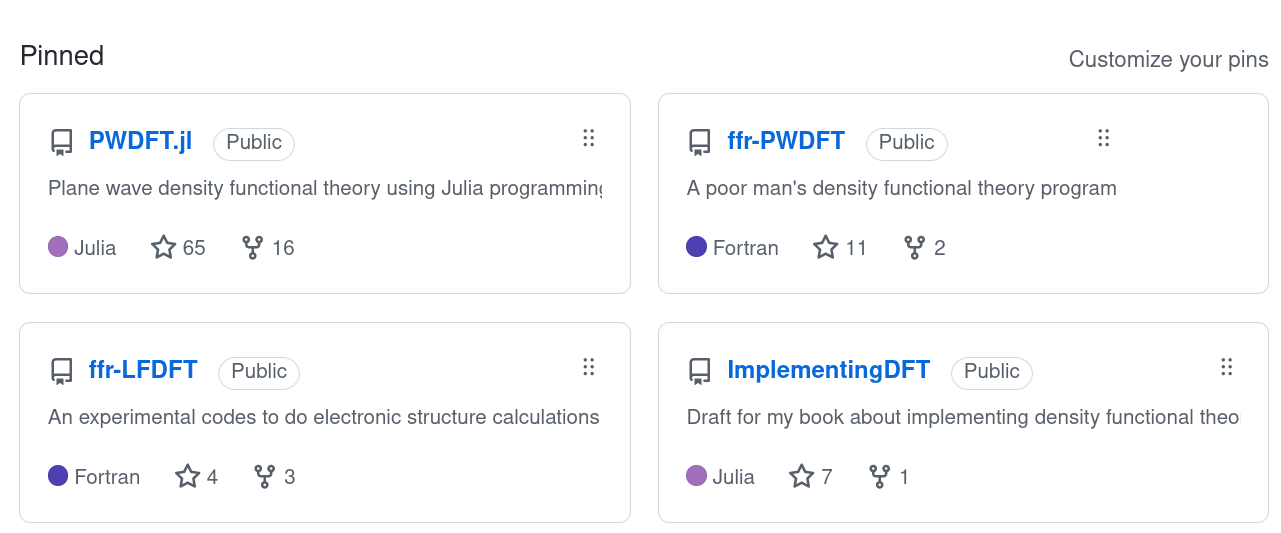
\includegraphics[width=\textwidth]{images/Github_ffr.png}
\par}

\end{frame}


%--------------------------------------------------------------
\begin{frame}
\frametitle{Wikipedia citation}

{\centering
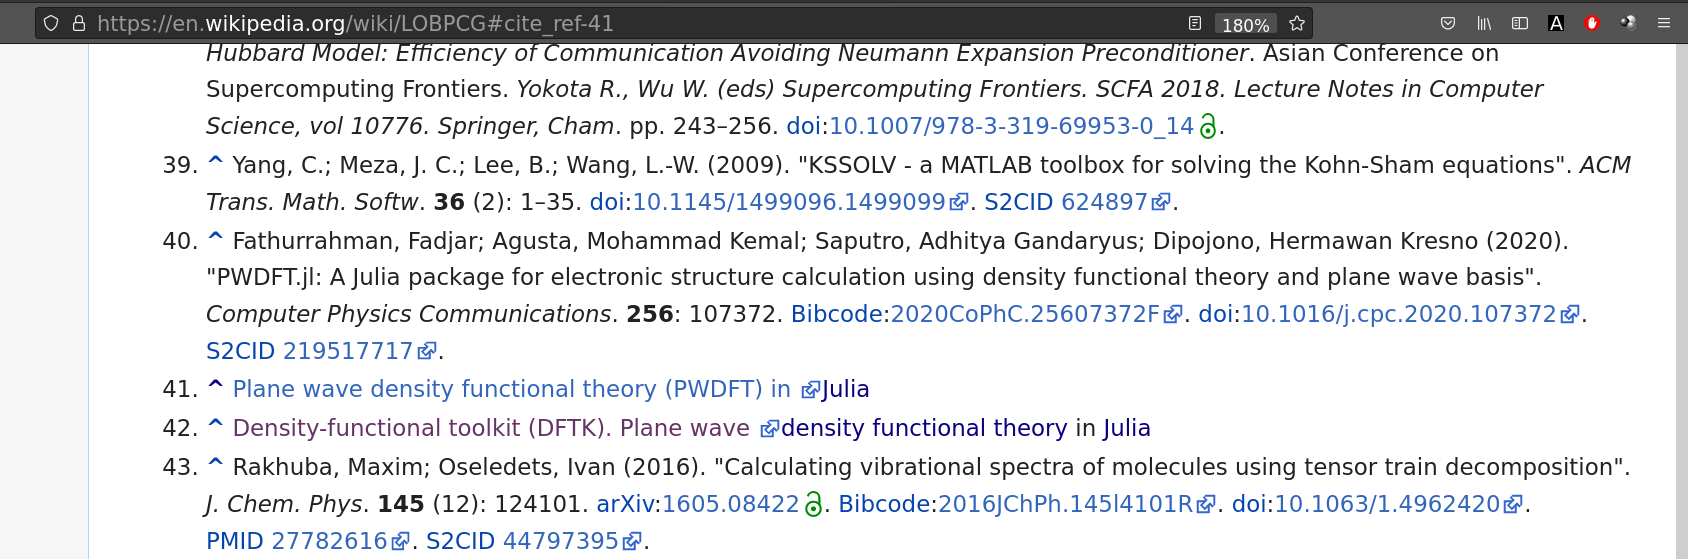
\includegraphics[width=\textwidth]{images/LOBPCG_wikipedia.png}
\par}

{\footnotesize
\url{https://en.wikipedia.org/wiki/LOBPCG\#cite_note-40}
}

\end{frame}


%--------------------------------------------------------------
\begin{frame}
\frametitle{Twitter mentions}

{\centering
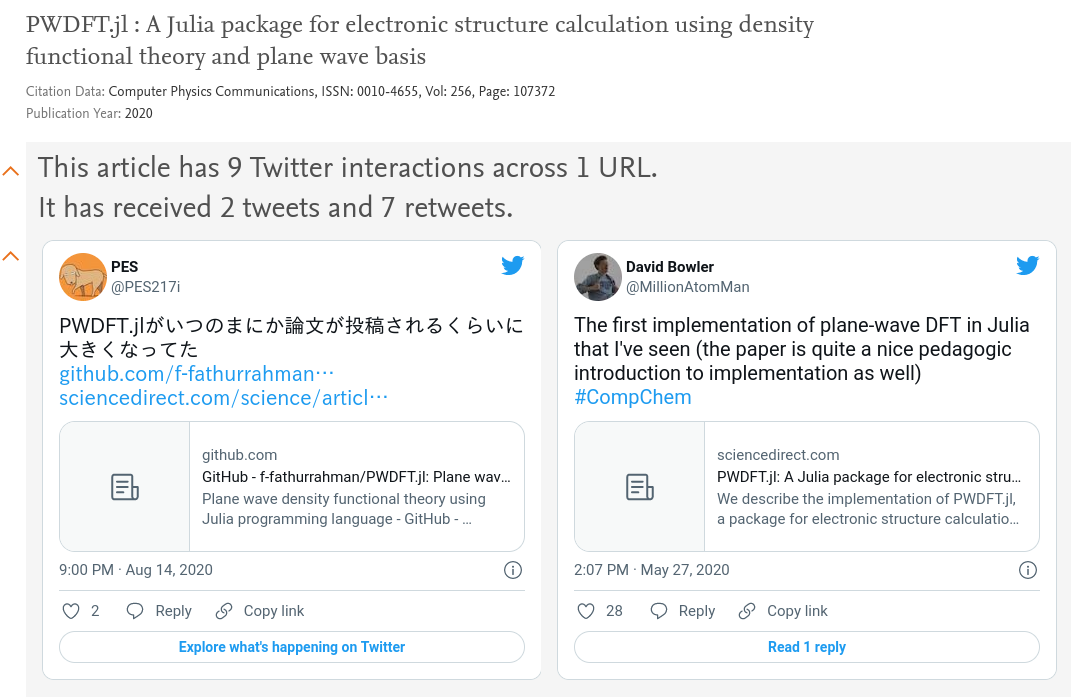
\includegraphics[width=0.7\textwidth]{images/Plumx_Tweet.png}
\par}

{\footnotesize
\url{https://plu.mx/plum/a/twitter?doi=10.1016/j.cpc.2020.107372}
}

\end{frame}


\end{document}

